\setboolean{IsHalfPage}{false}%
\setboolean{IsHalfPageLeftCol}{false}%
\setboolean{IsHalfPageRightCol}{false}%
\def\ChapterTitle{%
	Circular Hub
}
\def\ChapterUrl{%
	https://arnottferels.github.io/work/circular-hub
}
\def\ChapterDescription{%
	Lingkaran Hubung - Community Integration through Ecosystem, Culinary \& Education
}
\def\ChapterDetailsLine{%
	National Student Competition -- 2018 | Placemaking; Inclusive Design; Design Participatory  | Central Jakarta, Indonesia
}
\def\ChapterDetailsTabular{%
	\begin{tabular}{@{}ll}
		\textbf{Type}          & Professional Competition by Perumnas (National Urban Development Corporation) \\
		\textbf{Award}         & Top 10 \& Favorite                                                            \\
		\textbf{Contributions} & Research, Concept, Design, Modeling \& Visualization                          \\
		\textbf{Software}      & SketchUp, Lumion, Photoshop \& Illustrator                                    \\
		\textbf{Collaborators} & Steven Verdianta \& Billy Kurniawan                                           \\
		\textbf{URL}           & \textcolor{blue}{\footnotesize\texttt{\href{\ChapterUrl}{\ChapterUrl}}}       \\
	\end{tabular}
}
\def\ChapterAbstract{%
	This project signifies a transformative change at Jakarta's Kebon Melati Reservoir (KMR), establishing connections among communities through a circular design, inclusive culinary spaces, and versatile platforms. The primary objectives include boosting the local economy and addressing Nature Deficit Disorder, creating a harmonious environment for community growth.	Established in 1966, KMR holds a vital role in Jakarta, strategically positioned between slums and commercial areas, near landmarks like Grand Indonesia Mall, Thamrin Residence, and Mall. Serving as a connecting bridge, the reservoir dynamically transforms, reflecting the principles of Jurgen Habermas, the German philosopher.
}
\def\ChapterFrontmatter{%
	\chapter*{\ChapterTitle}\addcontentsline{toc}{chapter}{\ChapterTitle}
	\ChapterSetTocAddData{\ChapterDetailsLine}
	\ChapterSetDetailsData{\ChapterDescription}{\ChapterDetailsLine}{\ChapterDetailsTabular}
	\RuleAbstract%
	\ChapterAbstract
}
\StartTwoColumnLayout
\ChapterFrontmatter
\section*{
  Generate -- Inclusive Architectural Solutions for Community Enrichment
 }
\noindent
\begin{minipage}[t]{\linewidth}
	\hspace*{\fill}
	\begin{minipage}[t]{0.325\linewidth}
		%
\begin{figure}[H]
	\centering
	\includesvg[width=\linewidth]{src/graphics/circular-hub--generate-01.svg}
	\vspace{0.25cm}
	\caption*{%
		\parbox{0.8\linewidth}{%
			\raggedright
			\small
			\textcolor{black}{%
				\textnormal{%
					Creating a bridge using a ramp to connect various societies.
				}
			}
		}
	}
	\label{
		fig:circular-hub--generate-01
	}
\end{figure}

	\end{minipage}
	\begin{minipage}[t]{0.325\linewidth}
		%
\begin{figure}[H]
	\centering
	\includesvg[width=\linewidth]{src/graphics/circular-hub--generate-02.svg}
	\vspace{0.25cm}
	\caption*{%
		\parbox{0.8\linewidth}{%
			\raggedright
			\small
			\textcolor{black}{%
				\textnormal{%
					Developing a versatile platform for inclusive social and spatial activities.
				}
			}
		}
	}
	\label{
		fig:circular-hub--generate-02
	}
\end{figure}

	\end{minipage}
	\begin{minipage}[t]{0.325\linewidth}
		%
\begin{figure}[H]
	\centering
	\includesvg[width=\linewidth]{src/graphics/circular-hub--generate-03.svg}
	\vspace{0.25cm}
	\caption*{%
		\parbox{0.8\linewidth}{%
			\raggedright
			\small
			\textcolor{black}{%
				\textnormal{%
					Utilizing a circular shape to eliminate spatial boundaries.
				}
			}
		}
	}
	\label{
		fig:circular-hub--generate-03
	}
\end{figure}

	\end{minipage}
	\hspace*{\fill}
	\newline%
	\hspace*{\fill}
	\begin{minipage}[t]{0.325\linewidth}
		%
\begin{figure}[H]
	\centering
	\includesvg[width=\linewidth]{src/graphics/circular-hub--generate-04.svg}
	\vspace{0.25cm}
	\caption*{%
		\parbox{0.8\linewidth}{%
			\raggedright
			\small
			\textcolor{black}{%
				\textnormal{%
					Implementing an Inclusive Culinary Kiosk platform to boost the local community's economic condition around the KMR.
				}
			}
		}
	}
	\label{
		fig:circular-hub--generate-04
	}
\end{figure}

	\end{minipage}
	\begin{minipage}[t]{0.325\linewidth}
		%
\begin{figure}[H]
	\centering
	\includesvg[width=\linewidth]{src/graphics/circular-hub--generate-05.svg}
	\vspace{0.25cm}
	\caption*{%
		\parbox{0.8\linewidth}{%
			\raggedright
			\small
			\textcolor{black}{%
				\textnormal{%
					Implementing a shading roof for those on the move and establishing an area for thriving jasmine flowers.
				}
			}
		}
	}
	\label{
		fig:circular-hub--generate-05
	}
\end{figure}

	\end{minipage}
	\hspace*{\fill}
\end{minipage}
\vspace{1.0cm}%
\section*{
  Programs -- Ecosystem Integration for Community Enhancement
 }
\vspace{0.5cm}%
%
\begin{figure}[H]
	\centering
	\includesvg[width=\linewidth]{src/graphics/circular-hub--programs-01.svg}
	\label{
		fig:circular-hub--programs-01
	}
\end{figure}

\vfill
\columnbreak%
\begin{minipage}[t][\textheight][t]{\linewidth}
	\section*{
	  Programs -- Ecosystem Integration for Community Enhancement \textit{(cont.)}
	 }
	%
\begin{figure}[H]
	\centering
	\includesvg[width=\linewidth]{src/graphics/circular-hub--programs-02.svg}
	\label{
		fig:circular-hub--programs-02
	}
\end{figure}

	\vfill
	\section*{
	  Activities -- Holistic Platforms for Community Integration
	 }
	%
\begin{figure}[H]
	\centering
	\includesvg[width=\linewidth]{src/graphics/circular-hub--activities.svg}
	\label{
		fig:circular-hub--activities
	}
\end{figure}

	\vfill
	%
\begin{figure}[H]
	\centering
	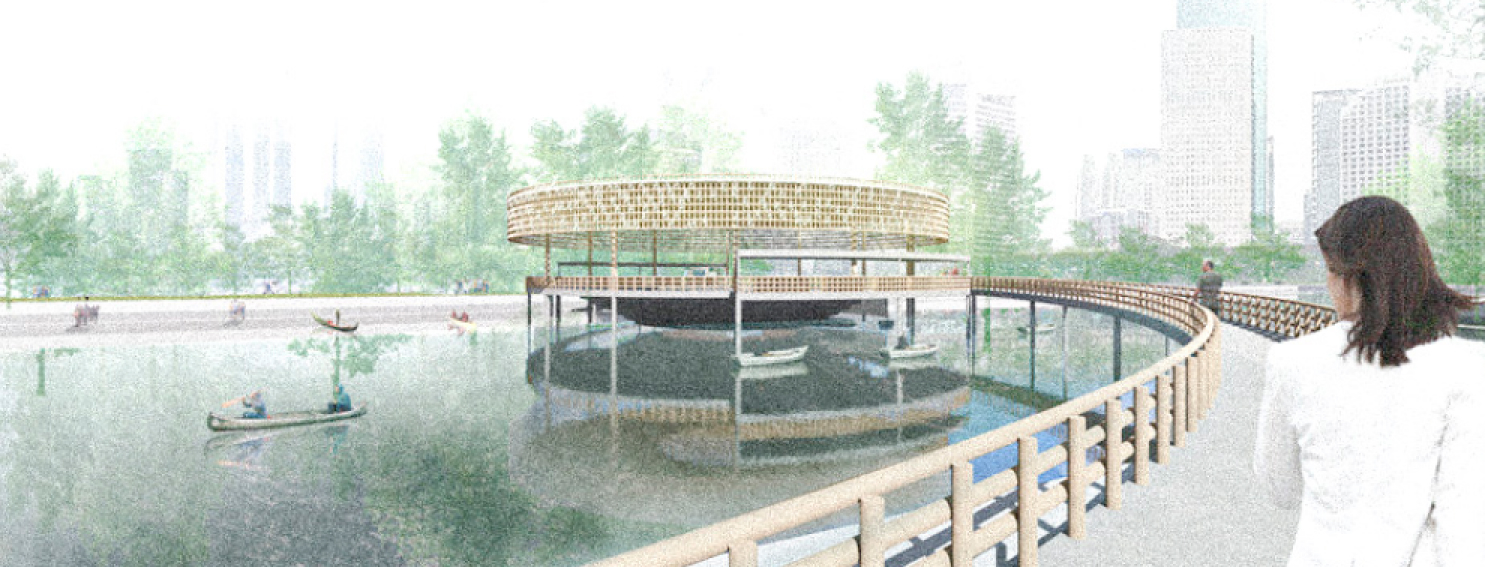
\includegraphics[width=\linewidth]{src/graphics/circular-hub--perspective.jpg}
	\label{
		fig:circular-hub--perspective
	}
\end{figure}

\end{minipage}
\EndTwoColumnLayout
\newpage
